
\subsubsection{22.10.14}

\begin{enumerate}
	\item Time of beginning and ending of congregation:
	18:00 - 21:40
	\item Purposes of congregation:
	\begin{enumerate}
	  \item To understand what causes the breakage of the guide.
	  
	  \item To repair the guide.
	  
	  \item To undersnand how to prevent this failure in the future.
	  
    \end{enumerate}
    
	\item Work, that has been done:
	\begin{enumerate}
	  \item After research of construction of the lift it was found that failure happened due to the excessive voltage due to the contraction of two guides by the transverse beam. It was decided to increase the distance between the guides replacing the layer between beam and guide to more thick nuts.
      
      \item To repair the slat failed so that it was replaced by the same.
      
      \begin{figure}[H]
      	\begin{minipage}[h]{1\linewidth}
      		\center{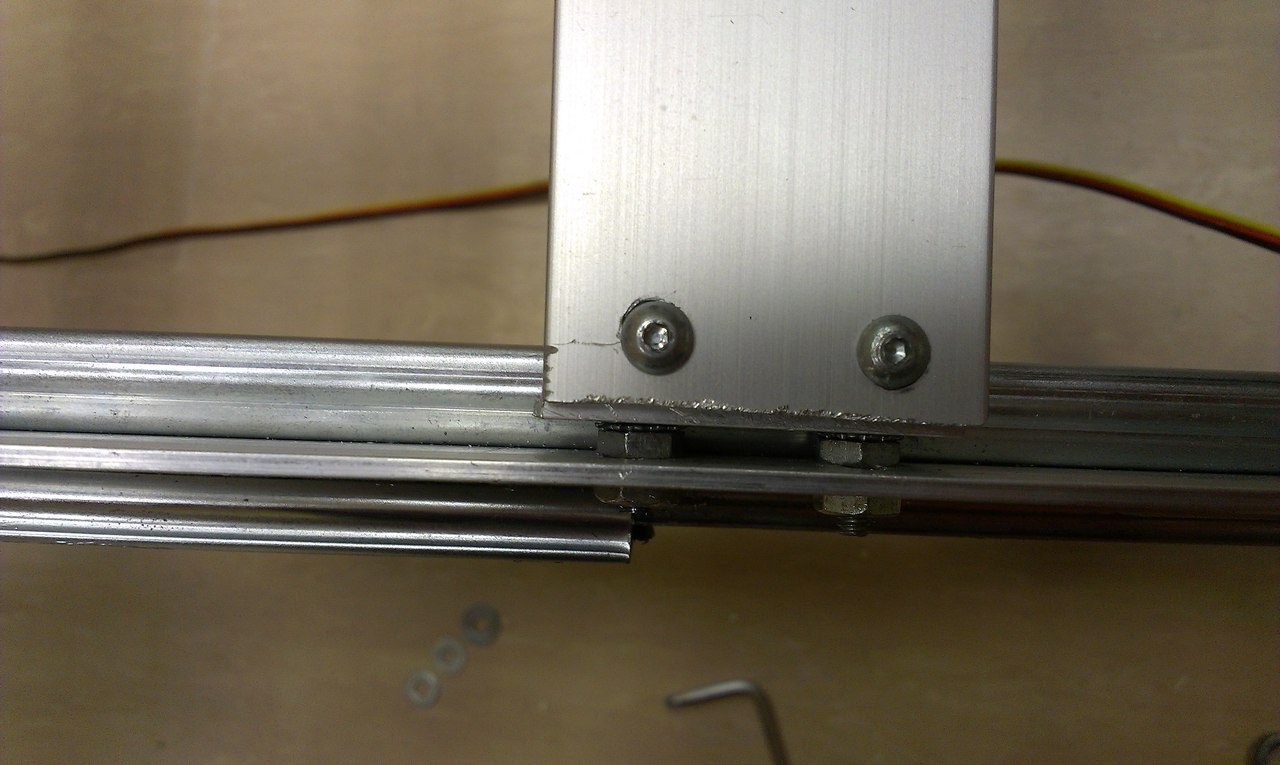
\includegraphics[scale=0.2]{days/22.10.14/images/01}}
      		\caption{Layer between beam and guide}
      	\end{minipage}
      \end{figure}
      
      \item It was decided to buy spare slats because to repair broken rakes it is impossible.
      
      \item In addition it was crated the mount for crossbar which will locate on the top slat.
      
      \begin{figure}[H]
      	\begin{minipage}[h]{1\linewidth}
      		\center{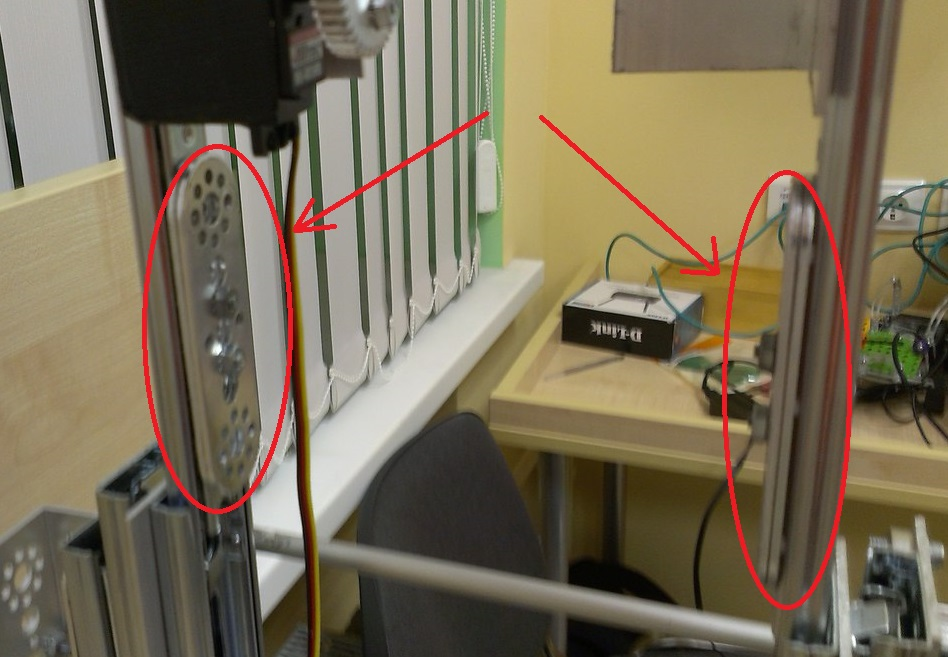
\includegraphics[scale=0.25]{days/22.10.14/images/02}}
      		\caption{Mount for crossbar}
      	\end{minipage}
      \end{figure}
      
    \end{enumerate}
    
	\item Result: 
	\begin{enumerate}
	  \item Repair of lift completed.
	  
      \item Created the mount for top crossbar.
      
    \end{enumerate}
    
	\item Tasks for the next congregations:
	\begin{enumerate}
	  \item Buy the spare furniture slats.
	  
    \end{enumerate}     
\end{enumerate}
\fillpage
